\documentclass[10pt,conference]{IEEEtran}
\usepackage{graphicx,booktabs,url}
\usepackage[T1]{fontenc}
\usepackage[utf8]{inputenc}
\begin{document}
\title{Human-Written vs. LLM-Generated TypeScript Projects: An Empirical Study}
\author{\IEEEauthorblockN{Simon Xie, Sukhdip Kandola, Thang To}\IEEEauthorblockA{CMPT 479 D100, School of Computing Science, Simon Fraser University, Burnaby, BC, Canada}}
\maketitle

\begin{abstract}
Coding agents now write whole repositories, yet comparisons of human and LLM code study single functions generated for benchmark tasks. We present an empirical study of \emph{whole TypeScript projects}: 36 human-written GitHub repositories pinned before 2021 and 36 repositories whose commits carry Claude Code's co-author signature, matched by project kind and size, plus 21 projects built by other agents (Codex, Copilot, Cursor, Devin, Jules, OpenHands). An automated, Docker-isolated pipeline installs each project from its own lockfile and measures compilation with its own \texttt{tsconfig}, lint violations under one shared ESLint/SonarJS rule set, complexity, duplication, structural testability from the import graph, and test effectiveness with the project's own tests and StrykerJS mutation testing. The main expectation we drew from prior work fails for all three questions. Agent-built projects have far fewer lint violations per KLOC (median 42.1 vs. 6.1, $\delta$~=~-0.93) and type-check cleanly more often (28/36 vs. 18/36), but their functions are more complex (mean cyclomatic complexity 1.76 vs. 2.83, $\delta$~=~+0.77). Their tests import more of the production code directly and pass far more often, while duplication, comment density and test-to-code ratio do not differ. Projects from six other agents show the same profile. Code, data and results are open source.
\end{abstract}
\begin{IEEEkeywords}
LLM-generated code, coding agents, TypeScript, empirical study, static analysis, mutation testing, testability
\end{IEEEkeywords}

\section{Introduction}
LLM coding agents such as Claude Code, Cursor and Codex now plan, write, test and commit entire projects. Code that compiles and looks plausible may still hide defects, poor practices or weak tests, so it matters whether agent-built software differs from software written by people. Prior comparisons study Python or Java \emph{functions} that researchers generated for benchmark tasks [2]--[4]. We instead study \emph{whole, real-world projects} written in TypeScript, an ecosystem with its own failure modes [1]. Python is only the language of our measurement pipeline. This is an \emph{empirical study}: we observe existing open-source projects rather than build a new analysis tool. We ask three questions, each with the expectation we derived from prior work before measuring:

\begin{itemize}
\item \textbf{RQ1 (code quality).} How do lint violations differ between human-written and LLM-generated TypeScript projects? \emph{Expectation:} more serious (problem-type) issues in LLM code, as [3] and [4] report for high-severity issues and unused constructs.
\item \textbf{RQ2 (complexity, maintainability, structural testability).} \emph{Expectation:} simpler LLM code [4], similar duplication, and tests that reach at least as much code, since agents write tests as they go [5].
\item \textbf{RQ3 (compilation).} Do LLM-generated projects have more compiler errors? \emph{Expectation:} yes, from hallucinated APIs and types.
\end{itemize}

Our contributions are a frozen, kind- and size-matched dataset of agent-built and human-written TypeScript projects with verified authorship, an open-source measurement pipeline, and the answers to RQ1--RQ3, including a check that the findings hold for agents other than Claude Code.

\section{Related Work}
\emph{Human vs. LLM code.} Molison et al. [2] ran SonarQube on human and LLM Python solutions at three difficulty levels. LLM code had fewer bugs and needed less effort to fix, but on competition-level tasks it introduced structural issues absent from the human solutions. Licorish et al. [3] analysed 72 Python tasks with Pylint, Radon and Bandit: GPT-4 code had more high-severity issues, while human code had more low-severity ones. Cotroneo et al. [4] compared over 500,000 Python and Java functions from humans and three LLMs. AI code was simpler and more repetitive, but had more unused constructs, hard-coded debugging and high-risk vulnerabilities. The three studies therefore agree that LLM code is \emph{not uniformly worse}: it has fewer minor issues, and its risks concentrate in rarer, more serious ones that grow with task difficulty. They disagree on bug counts: [2] finds fewer bugs, [3] more severe issues. All three share one design, which is researcher-generated, function-level code in Python or Java.

\emph{Tests and mutation.} TestPilot [5] showed that an LLM can write JavaScript unit tests with a median 70\% statement coverage, so agent-built projects plausibly ship with substantial tests. Mutation testing measures whether such tests catch faults. LLMorpheus [6] found that LLM-written mutants capture bugs StrykerJS misses, and CDBench [7] found that LLMs write useful tests but often invalid mutants. Garg et al. [8] showed that SWE-Bench overstates agent ability, including on TypeScript, when task descriptions are unrealistic. Bruntink and van Deursen [9] linked a unit's size and fan-out to the test effort it needs, which we use as structural testability. \emph{Gap:} no study compares \emph{whole projects} that coding agents actually built and published with human projects, in TypeScript, on compilation, quality, structure and test effectiveness together. We fill that gap.

\section{Study Design}
\subsection{Dataset}
\emph{Discovery.} Candidates come from the GitHub search API (\texttt{bench/discover.py}) by two routes: README phrases that advertise agent-built development, and the commit index searched for nine agents' own signatures. This gave 1,236 and 1,409 candidates. A screening stage (\texttt{bench/screen.py}) applies fixed rules to each: a root \texttt{package.json} and \texttt{tsconfig.json}, a real \texttt{test} script, no workspaces, $\geq$60\% TypeScript, and 40~KB--1.5~MB of TypeScript. Projects without tests are therefore excluded up front, because RQ2 needs a suite to measure.

\emph{Authorship evidence.} A creation date after 2023 does not prove AI authorship, so the LLM group requires positive evidence. \texttt{bench/authorship.py} detects ten agents' co-author trailers and bot authors, and a project is eligible only if $\geq$50\% of its last 100 commits carry one. This removed 779 of 1014 self-described LLM candidates. The selected projects have a median of 79\% agent-signed commits (a lower bound). Human projects are pinned to their last commit before 2021-01-01, which predates Copilot's preview and ChatGPT.

\emph{Selection and matching} (\texttt{bench/select\_repos.py}). The LLM group is every eligible project whose main agent is Claude Code (36). Each is paired with an unused eligible human project ($\geq$100 stars) by a cost of |log size ratio|, plus ln~2 when the project kinds differ (library, CLI, service, UI app or extension, read from \texttt{package.json}). 20 of 36 pairs share a kind. LLM projects are larger (median human/LLM size ratio 0.45), because few large human projects pass screening, so every count is normalised per KLOC and we test for size effects (Sec.~IV-D). The 21 projects built mainly by other agents (Codex, Copilot, Cursor, Devin, Jules, OpenHands) form a third, unmatched group. \texttt{dataset/repos.csv}, \texttt{repos\_agents.csv} and \texttt{pairs.csv} freeze every commit analysed.

\subsection{Pipeline and measures}
Each repository is cloned at its pin and copied into a fresh container of one Docker image (Node~22, pinned tools). Dependencies are installed with the project's own package manager and lockfile, and its own TypeScript version checks its own \texttt{tsconfig.json} (RQ3). Every project is linted with \emph{one} shared ESLint~9 configuration (typescript-eslint and SonarJS recommended rules), ignoring its own disable comments; each violation is typed \emph{problem} or \emph{suggestion} (RQ1). RQ2 uses per-function cyclomatic [10] and cognitive [11] complexity, jscpd duplication and comment density. For \emph{structural testability} (\texttt{bench/testability.py}) we build each project's import graph and measure internal fan-out per module [9], the share of production code that a test imports directly, and the share a test can reach transitively. \emph{Test effectiveness} runs the project's own \texttt{test} script (15-minute limit) and, where it passes, StrykerJS mutation testing on a seeded sample of up to 10 production files. Suites that fail are re-run on a Node version from the project's era; a suite that cannot run counts as 0\% passing and gets no mutation score. All counts are per KLOC of production code.

\subsection{Analysis plan}
The primary test compares the human and Claude Code groups with two-sided Mann--Whitney U tests, Cliff's~$\delta$ as effect size (magnitudes per [12]) and Holm correction [13] across the 22 metrics. Robustness checks are (i) Wilcoxon signed-rank tests over the matched pairs, (ii) a rank regression on group and log size, (iii) human vs. all 57 agent-built projects, and (iv) other agents vs. each group. With 36 projects per group the test has 80\% power for |$\delta$|~$\geq$~0.38, against 0.64 with the 12 per group of our milestone.

\section{Results}
\begin{table}[t]
\caption{Medians per group. $\delta$: Cliff's delta, Claude Code vs. human (+: higher in Claude Code). p: Holm-corrected Mann--Whitney U (Fisher exact for compiling). p pair: Holm-corrected Wilcoxon over matched pairs. Bold: p \textless{} 0.05}
\label{tab:results}
\centering
\scriptsize
\setlength{\tabcolsep}{2.5pt}
\begin{tabular}{lcccccc}
\toprule
Metric (RQ) & Human & Claude & Other & $\delta$ & p & p pair \\
\midrule
Lint violations/KLOC (1) & 42.1 & 6.1 & 5.8 & -0.93 & \textless{}0.001 & \textless{}0.001 \\
Problem violations/KLOC (1) & 9.6 & 1.8 & 0.8 & -0.81 & \textless{}0.001 & \textless{}0.001 \\
Era-neutral viol./KLOC (1) & 16.6 & 6.1 & 5.7 & -0.59 & \textless{}0.001 & \textless{}0.001 \\
Explicit \texttt{any}/KLOC (1) & 14.2 & 0.0 & 0.0 & -0.87 & \textless{}0.001 & \textless{}0.001 \\
Mean cyclomatic CC (2) & 1.76 & 2.83 & 3.13 & +0.77 & \textless{}0.001 & \textless{}0.001 \\
\% functions CC\textgreater{}10 (2) & 0.1 & 3.9 & 4.3 & +0.87 & \textless{}0.001 & \textless{}0.001 \\
\% functions cogn.\textgreater{}15 (2) & 0.0 & 1.4 & 1.9 & +0.57 & \textless{}0.001 & \textless{}0.001 \\
Functions/KLOC (2) & 97 & 80 & 62 & -0.24 & 0.755 & 1.000 \\
Duplicated lines \% (2) & 0.44 & 0.55 & 1.51 & -0.01 & 1.000 & 1.000 \\
Comment density (2) & 0.086 & 0.109 & 0.023 & +0.13 & 1.000 & 1.000 \\
Internal fan-out/module (2) & 2.10 & 2.53 & 2.10 & +0.21 & 0.950 & 1.000 \\
\% code tested directly (2) & 22 & 55 & 35 & +0.40 & 0.040 & 0.175 \\
\% code reached by tests (2) & 70 & 72 & 42 & +0.10 & 1.000 & 1.000 \\
Test-to-code ratio (2) & 0.33 & 0.54 & 0.22 & +0.17 & 1.000 & 1.000 \\
Test pass rate (2) & 0.01 & 1.00 & 1.00 & +0.48 & 0.001 & 0.001 \\
Mutation score (2) & 0.43 & 0.26 & 0.15 & -0.30 & 1.000 & 1.000 \\
tsc errors/KLOC (3) & 0.00 & 0.00 & 0.06 & -0.03 & 1.000 & 1.000 \\
Compiles cleanly (3) & 18/36 & 28/36 & 9/21 &  & 0.026 &  \\
Own tests pass (2) & 13/36 & 29/36 & 13/21 &  &  &  \\
\bottomrule
\end{tabular}
\end{table}

Table~I summarises all metrics. 13 of 22 differ significantly between the human and Claude Code groups after Holm correction, and 12 in the paired test. Fig.~1 shows the per-project spread for six of them, including the other-agent group.

\begin{figure}[t]
\centering
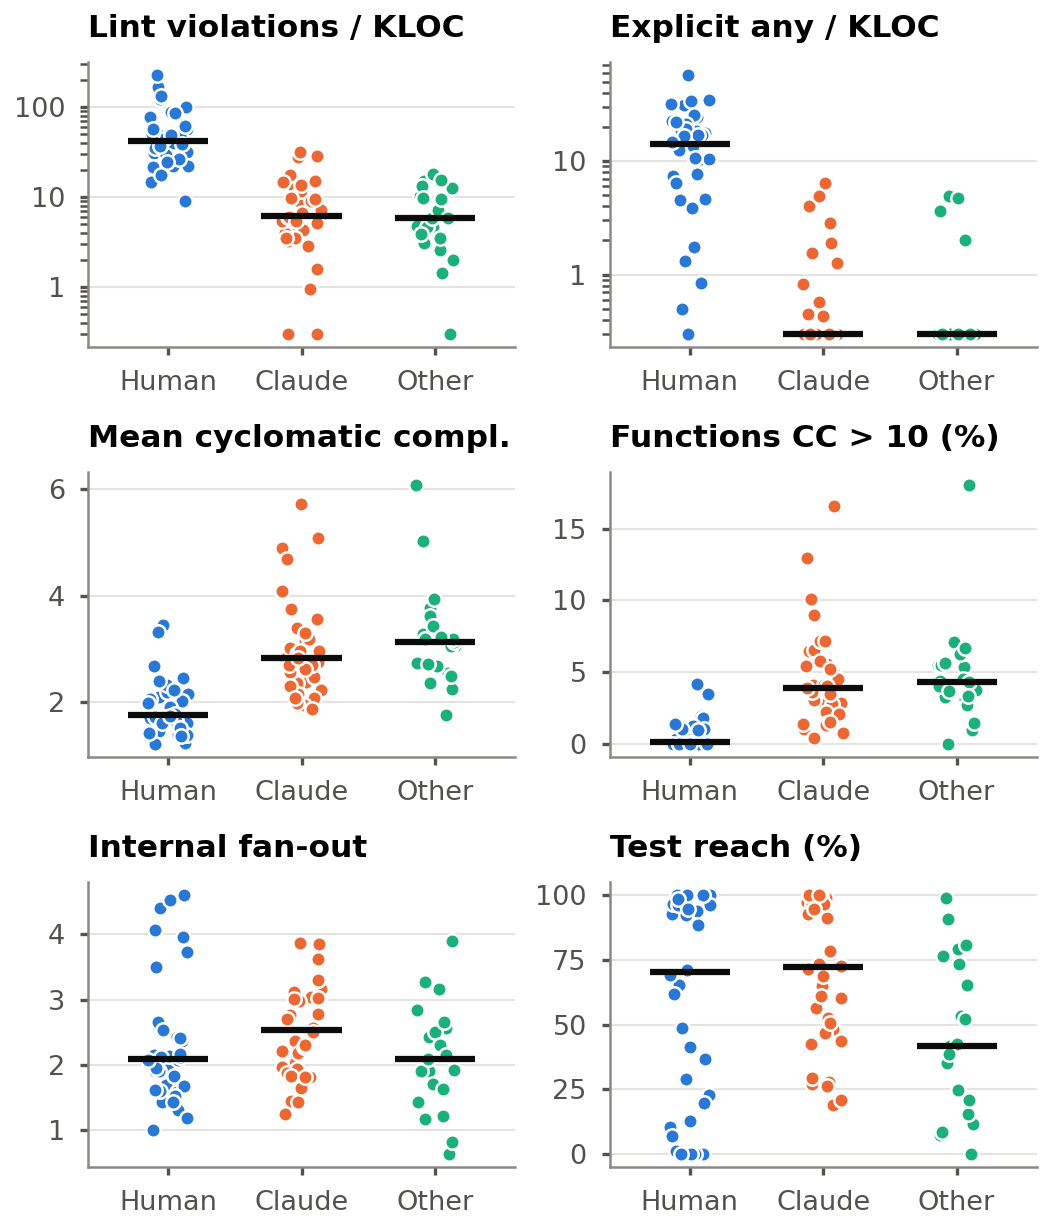
\includegraphics[width=\columnwidth]{figures/metrics_by_agent_group.png}
\caption{Per-project values for human, Claude Code and other-agent projects (dots) with group medians (bars). Violation panels use a log axis, with zero-violation projects drawn at its floor.}
\label{fig:groups}
\end{figure}

\subsection{RQ1: Code quality}
Contrary to our expectation, Claude Code projects have far \emph{fewer} violations: 42.1 vs. 6.1 per KLOC ($\delta$~=~-0.93, Holm \emph{p}~\textless{}~0.001), and fewer \emph{problem}-type ones (9.6 vs. 1.8, $\delta$~=~-0.81). Human code is dominated by \texttt{no-explicit-any}, \texttt{no-unused-vars}, \texttt{prefer-const}; explicit \texttt{any} alone has a median of 14.2 vs. 0.0 per KLOC. LLM code is dominated by \texttt{no-nested-conditional}, \texttt{cognitive-complexity}, \texttt{no-unused-vars}, which are structural rather than typing issues. Part of the gap is an \emph{era effect}, since older TypeScript lacked \texttt{unknown} and commonly used \texttt{var} and \texttt{require}. Excluding 12 era-dependent rules still leaves 16.6 vs. 6.1 ($\delta$~=~-0.59, Holm \emph{p}~\textless{}~0.001). The result agrees with Molison et al. [2] rather than [3], [4]: we found no sign of more serious issues in LLM projects.

\subsection{RQ2: Complexity, maintainability and testability}
Here the expectation from [4] is reversed. Claude Code functions are \emph{more} complex: mean cyclomatic complexity 1.76 vs. 2.83 ($\delta$~=~+0.77, Holm \emph{p}~\textless{}~0.001), 0.1 vs. 3.9\% of functions above McCabe's threshold of 10, and 0.0 vs. 1.4\% above Sonar's cognitive threshold of 15 ($\delta$~=~+0.57). Functions per KLOC do not differ significantly (97 vs. 80), so agent code branches and nests more rather than merely packing more code into each function. Duplication (0.44 vs. 0.55), comment density (0.086 vs. 0.109) and test-to-code ratio (0.33 vs. 0.54) do not differ (Holm \emph{p}~=~1.000, \emph{p}~=~1.000, \emph{p}~=~1.000).

\emph{Structural testability} is mixed. Internal fan-out does not differ (2.10 vs. 2.53 project modules imported per module, Holm \emph{p}~=~0.950), but Claude Code modules import fewer external packages (1.25 vs. 0.79, $\delta$~=~-0.44, Holm \emph{p}~=~0.014), so their units have fewer dependencies to stub. Their tests import 22 vs. 55\% of production code directly ($\delta$~=~+0.40, Holm \emph{p}~=~0.040; paired \emph{p}~=~0.175), yet the share reachable from any test is similar (70 vs. 72\%, Holm \emph{p}~=~1.000): human suites reach code through a few entry points, agent suites test modules one by one.

\emph{Test effectiveness.} Own suites pass on Node~22 for 29/36 Claude Code projects but 13/36 human ones. Re-running every failing human suite on a Node version from its era rescued only 1. We diagnosed each failure from its logs (\texttt{dataset/test\_failure\_causes.csv}): 21 of 23 failing human suites have \emph{decayed} (dependency rot, a needed browser or service, undeclared tools, missing build output) and 2 fail on assertions, whereas 5 of 7 failing Claude Code suites are genuine assertion failures. Mutation testing gave a valid score for 8 human and 23 Claude Code projects (medians 0.43 vs. 0.26, Holm \emph{p}~=~1.000); Stryker's instrumented code broke the old Jest set-up of 3 further human projects. Because mutation needs a passing suite, this comparison is small and descriptive.

\subsection{RQ3: Compilation}
Installation succeeded for 33/36 human and 36/36 Claude Code projects. With each project's own compiler and configuration, 28/36 Claude Code and 18/36 human projects type-check with no errors (Fisher \emph{p}~=~0.026); counting only errors in project files, 28/36 and 27/36 are clean. Errors per KLOC in project files do not differ (0.00 vs. 0.00, Holm \emph{p}~=~1.000). The answer to RQ3 is \emph{no}: LLM projects do not have more compilation errors, and compile cleanly more often. Most human errors come from decay (unresolvable packages, today's \texttt{@types} written in syntax the pinned compiler cannot parse), whereas the few LLM errors are genuine type or configuration mistakes.

\subsection{Robustness and other agents}
The differences are not size effects: in a rank regression on group and log KLOC, 13 metrics keep a significant group effect after Holm correction, including lint violations (\emph{p}~\textless{}~0.001) and mean cyclomatic complexity (\emph{p}~\textless{}~0.001). The paired test over matched projects agrees (12 metrics), and so does pooling all 57 agent-built projects against the human group (12 metrics). The 21 other-agent projects differ from human projects on 12 metrics and from Claude Code on one (comment density); 9/21 type-check cleanly (vs. Claude Code: Fisher \emph{p}~=~0.011). Their tests reach less code (median 42\%), and mutation testing scored only 6 of them.

\section{Discussion and Limitations}
\emph{Interpretation.} Agent-built projects look \emph{cleaner} by every rule-based measure: fewer lint violations, almost no explicit \texttt{any}, clean compiles and passing tests. Agents run linters, type-checkers and tests in their own loop, and they write modern idioms. Much of the human disadvantage, however, is \emph{decay}: four to eight years of ecosystem drift break installs, types and suites that once worked. Whether agent-built projects decay more slowly is an open question that only time can answer. Where agents are clearly worse is \emph{complexity}: their functions branch and nest more. This reconciles prior work. Function-level studies find generated code simpler [4] because a benchmark function is small, whereas an agent building a whole feature concentrates logic in fewer, deeper functions, which matches the structural issues on hard tasks in [2]. For reviewers, complexity rather than lint is the place to look. Agents also write per-module unit tests, as TestPilot-style generation suggests [5], but those tests do not kill more mutants.

\emph{Threats to validity.} (Construct) Co-author trailers show that an agent took part in commits, not that it wrote every line, so the LLM group is \emph{agent-assisted}; our testability measures are static import reachability, not coverage. (Internal) The human group is necessarily older. Era-neutral rules, era-matched test re-runs and the failure diagnosis control for part of this, and a contemporary human group cannot be verified AI-free. (External) LLM projects are younger, less starred and larger than their human matches, and the other-agent group is small and unmatched. The results describe screened single-package projects with tests, not all TypeScript. (Conclusion) We report effect sizes, Holm-corrected and paired tests; the mutation comparison is underpowered.

\section{Conclusion}
Across 93 TypeScript projects, agent-built code is not the low-quality code our reading of function-level studies led us to expect. It has far fewer lint violations, compiles at least as reliably, and its tests pass and target modules directly, but its functions are more complex. The same profile holds for six other agents. Future work should generate matched projects from the same specifications with open models, and follow agent-built projects over time to see whether they decay. The pipeline, dataset and raw results are at \texttt{github.com/tothang28012001/ts-llm-benchmark}.

\begin{thebibliography}{99}
\bibitem{r1} T. Tang, S. Alimadadi, and N. Sumner, “From logic to toolchains: An empirical study of bugs in the TypeScript ecosystem,” in \emph{Proc. 23rd Int. Conf. Mining Software Repositories (MSR)}, ACM, 2026, pp. 539--549.
\bibitem{r2} A. S. Molison, M. Moraes, G. Melo, F. Santos, and W. K. G. Assunção, “Is LLM-generated code more maintainable \& reliable than human-written code?” in \emph{Proc. ACM/IEEE Int. Symp. Empirical Software Engineering and Measurement (ESEM)}, 2025, pp. 151--162.
\bibitem{r3} S. A. Licorish, A. Bajpai, C. Arora, F. Wang, and K. Tantithamthavorn, “Comparing human and LLM generated code: The jury is still out!” arXiv:2501.16857, 2025.
\bibitem{r4} D. Cotroneo, C. Improta, and P. Liguori, “Human-written vs. AI-generated code: A large-scale study of defects, vulnerabilities, and complexity,” in \emph{Proc. 36th IEEE Int. Symp. Software Reliability Engineering (ISSRE)}, 2025, pp. 252--263.
\bibitem{r5} M. Schäfer, S. Nadi, A. Eghbali, and F. Tip, “An empirical evaluation of using large language models for automated unit test generation,” \emph{IEEE Trans. Software Engineering}, vol. 50, no. 1, pp. 85--105, 2024.
\bibitem{r6} F. Tip, J. Bell, and M. Schäfer, “LLMorpheus: Mutation testing using large language models,” \emph{IEEE Trans. Software Engineering}, vol. 51, no. 6, pp. 1645--1665, 2025.
\bibitem{r7} A. Romazanov, G. Fraser, and S. Herbold, “CDBench: Benchmarking the mutation testing capabilities of LLMs with Code Defenders,” \emph{Empirical Software Engineering}, vol. 31, no. 6, art. 166, 2026.
\bibitem{r8} S. Garg, B. Steenhoek, and Y. Huang, “Saving SWE-Bench: A benchmark mutation approach for realistic agent evaluation,” in \emph{Proc. 5th IEEE/ACM Int. Conf. AI Engineering -- Software Engineering for AI (CAIN)}, 2026.
\bibitem{r9} M. Bruntink and A. van Deursen, “An empirical study into class testability,” \emph{J. Systems and Software}, vol. 79, no. 9, pp. 1219--1232, 2006.
\bibitem{r10} T. J. McCabe, “A complexity measure,” \emph{IEEE Trans. Software Engineering}, vol. SE-2, no. 4, pp. 308--320, 1976.
\bibitem{r11} G. A. Campbell, “Cognitive complexity: An overview and evaluation,” in \emph{Proc. Int. Conf. Technical Debt (TechDebt)}, 2018, pp. 57--58.
\bibitem{r12} J. Romano, J. D. Kromrey, J. Coraggio, and J. Skowronek, “Appropriate statistics for ordinal level data,” in \emph{Proc. Annual Meeting of the Florida Association of Institutional Research}, 2006.
\bibitem{r13} S. Holm, “A simple sequentially rejective multiple test procedure,” \emph{Scandinavian J. Statistics}, vol. 6, no. 2, pp. 65--70, 1979.
\bibitem{r14} StrykerJS, https://stryker-mutator.io; ESLint, https://eslint.org; typescript-eslint, https://typescript-eslint.io; SonarJS, https://github.com/SonarSource/SonarJS; jscpd, https://github.com/kucherenko/jscpd.
\end{thebibliography}
\end{document}
